\documentclass[journal, compsoc]{IEEEtran}
%\documentclass[12pt, journal, compsoc,onecolumn]{IEEEtran}
%\linespread{1.5}

%\documentclass[12pt]{article}
\usepackage[monochrome]{color}

%bibliography style
\usepackage[numbers]{natbib}

% input encoding
\usepackage[utf8]{inputenc}

% PDF figures
\usepackage[pdftex]{graphicx}
\DeclareGraphicsExtensions{.pdf,.png,.jpg,.jpeg,.PNG,.JPG,.JPEG}

% additional packages
\usepackage{url}

% set PDF version to 1.6
\pdfminorversion=6

%acronyms
\usepackage[printonlyused,withpage]{acronym}


% http://texblog.org/2011/02/26/generating-dummy-textblindtext-with-latex-for-testing/
\usepackage[english]{babel}
\usepackage{blindtext}

%listings (code blocks)
\usepackage{listings}
\usepackage{xcolor}

\definecolor{mygreen}{rgb}{0,0.6,0}
\lstset{ %
  basicstyle=\footnotesize\ttfamily,        % the size of the fonts that are used for the code
% breakatwhitespace=true,          % sets if automatic breaks should only happen at whitespace
  breakindent=1em,
  breaklines=true,                 % sets automatic line breaking
  commentstyle=\color{mygreen},  % comment style
  keepspaces=true,                 % keeps spaces in text, useful for keeping indentation of code (possibly needs columns=flexible)
  %keywordstyle=\color{blue},       % keyword style
  %linewidth=\textwidth,
  %morekeywords={*,...},            % if you want to add more keywords to the set
  %numbers=left,                    % where to put the line-numbers; possible values are (none, left, right)
  %numbersep=5pt,                   % how far the line-numbers are from the code
  %numberstyle=\tiny\color{gray},   % the style that is used for the line-numbers
  showlines=true,
  stepnumber=1,                    % the step between two line-numbers. If it's 1, each line will be numbered
  %stringstyle=\color{red},         % string literal style
  %tabsize=2,                       % sets default tabsize to 2 spaces
  title=\lstname                   % show the filename of files included with \lstinputlisting; also try caption instead of title
}


\begin{document}% max 10 pages,

\title{Project Level Effects of Gender on Contribution Evaluation on GitHub}

\author{
	\IEEEauthorblockN{Pascal Brokmeier (B.Sc.)}\\
	\IEEEauthorblockA{Universität zu Köln, Germany}\\
	\IEEEauthorblockA{pbrokmei@smail.uni-koeln.de}
	}

\maketitle

\begin{abstract}% max 150 words

Distributed open source software development has largely turned to GitHub, a pull-based software development collaboration platform. Recent studies have deployed data science techniques on the large datasets available about millions of projects on GitHub. Some research has focused on \ac{PR} acceptance predictors and some evidence was found of sexual discrimination among members, more specifically in the probability of acceptance of \ac{PR}s by different genders. In this paper we analyzed the influence of gender on \ac{PR} acceptance on a project level, comparing different popular projects regarding their discrimination factors. Several projects were identified that have significant differences between male and female \ac{PR} acceptance rates.
\end{abstract}

%\begin{IEEEkeywords}
% a, b, c
%\end{IEEEkeywords}

\section{Introduction}\label{Introduction}

%\subsection{Background}%TODO delete
\IEEEPARstart{S}{oftware} development has adapted to the needs for distributed development through the concepts of social coding and pull based software development pushed by platforms like GitHub which provide a platform for some of the biggest \ac{OSS} projects existing. Projects like rails, docker, angular, node or swift are publicly hosted with some of them having thousands of followers and contributors. Open Source software development has been described as meritocracies \cite{Scacchi:2007:FSS:1295014.1295019}, however recent research has identified social factors to influence decisions of project managers. This holds also true for the acceptance of contributions by others through \ac{PR}s. \cite{Tsay:2014:IST:2568225.2568315}. Inevitably, a social coding environment such as GitHub is accompanied with social interaction that influences the project progress.

%\subsection{Motivation}%TODO delete
An obvious factor in social interaction is gender. Research has shown that women are being treated unequal in professional environments, receive promotions less likely than men and are less likely to be hired when compared to male competition \cite{Davison2000225, doi:10.1177/0149206310374774}.
and more specifically \ac{OSS} projects have been shown to exhibit sexist behavior. About 1.5\% of the total number of members in communities of \emph{'\ac{F/LOSS}'} were determined to be female compared to 28\% in proprietary software as determined in a 2005 report by the University of Cambridge \cite{flosspols-gender:2005}. More current research shows a percentage of about 9\% female users on GitHub \cite{Vasilescu:2015:GTD:2702123.2702549}.

\citeauthor{10.2307/23443867} found equal gender mix teams to perform better than male or female dominated teams in the context of business students. Increased mutual monitoring, a form of informal Clan Control \cite{doi:10.1287/orsc.7.1.1}, was found to be a strong beneficial factor in mixed gender teams.

\citeauthor{Vasilescu:2015:GTD:2702123.2702549} more specifically found gender diversity to have beneficial effects on \ac{OSS} team performance. This creates an economic incentive for organizations to promote diversity in their teams and communities.

\citeauthor{Tsay:2014:IST:2568225.2568315} found project managers to use social cues to evaluate contributions and \citeauthor{Vasilescu:2015:GTD:2702123.2702549} found almost half of the project members to be aware of other users gender. Consequently the effect of the perceived gender on this contribution process can be of interest in the ongoing debate of gender inequality. Current research performed by \citeauthor{genderdiff:2016} has identified a significant difference between the acceptance rate of \ac{PR}quests created by men and women. Women whose profile publicly display their gender have a 4.1\% lower chance of their \ac{PR} being accepted compared to mens and a 10\% lower chance than those women that did not disclose their gender. This is especially interesting as this percentage only holds true for 'visible'
%TODO all ' " "'
women. Those that decided to withhold information about their gender in their profile have a higher chance of having their request accepted.


In their research, \citeauthor{genderdiff:2016} have analyzed a variety of different topology factors on the dataset. They have analyzed their results for different biases most notably an extensive covariate analysis which showed no explanations for the bias towards men. They also analyzed different programming languages and their relation to the acceptance rates. They however did not compare gender-dependent acceptance rates on a project level, allowing project specific environment and culture to explain the discovered differences.

%\subsection{Research Question}%TODO delete
These factors, the underrepresentation of women on GitHub, the observed sexist behavior within \ac{OSS} communities as well as the social influences on decisions that were believed to be purely lead by meritocratic reasoning raise the following question:%two questions:

\emph{Can project level differences in acceptance rates of \ac{PR}s between genders be observed on GitHub?}
%\emph{What factors can explain these differences?}
%TODO Nils: Too generic. focus on specific factors. what project specific factors do I want to focus on?
%\emph{How does the perceived gender affect the evaluation of contributions by members in a public social coding environment such as GitHub?}

%If significant differences on a project level can be observed, the obvious next question is what factors might cause these differences.

%Method, process explaination
%\subsection{Research Method}
To answer the research question and due to the large amount of data accessible, data analytics techniques need to be applied. To ensure sufficient data is available per project, the biggest 100 projects on GitHub are selected
\footnote{the projects were sorted based on their stars which is a good proxy for their popularity and therefore their community size}.

This paper quantitatively analyzes differences of gender participation between projects. It does not try to determine the relevance of gender in comparison to other social cues in the process of deciding whether to merge or decline a \ac{PR}. Instead, this work is looking for project level differences in gender dependent \ac{PR} statistics. %evaluate if I also do the qualitative part or only the quantitative part.

The structure of the paper is as follows: First, some background on gender inequality research in professional settings and more specifically in \ac{OSS} will be provided. Afterwards, general research on GitHub data is reviewed and the most recent research of gender influences on GitHub will be introduced. In the next chapter, the research method and data acquisition will be described to facilitate the reproducibility of this work. Subsequently the results will be presented and discussed. Finally limitations and ideas for further research complete the paper.
%TODO QUALITATIVE
%Based on the data collected, outlier projects can then be further analyzed with qualitative methods to determine the reasons of the differences in gender participation.

%\begin{itemize}
    %\item How can the perceived gender for each user be determined? What is the perceived gender for each user?
    %\item When is a contribution considered to be accepted? When is it considered to be rejected?
    %\item Is a correlation existing between gender of the contributor and the contribution evaluation result? Can causal identification be achieved?% "causal identification?" sounds shitty
%\end{itemize}

%The first two tasks need to be resolved using proper technical analysis of the data and using data such as followers as proxies for social standing and network embeddedness. The last task is reliant on the results of the first two as well as the methods available to us to achieve causal identification such as \ac{RCA}. While a simple correlation would already be of interest, discovering a causal effect would be more satisfying.

%To analyze the data, the GHTorrent \cite{Gousi13} dataset is used, which allows the execution of queries against a huge dataset of all repositories, users, \ac{PR}s, comments and issues on GitHub since 2013. The dataset included over 14 million users and 13 million \ac{PR}s in November 2016 although the number of relevant users is expected to be much lower since the distribution of active users is a long tail distribution with very few active users and many inactive or abandoned accounts. Nonetheless, the scale of the dataset allows for thorough data preprocessing without loosing too many potential entries for the analysis afterwards.


%TODO do I do merge analysis on commit level or not?
%Since \ac{PR} are hard to determine as either merged or not merged however, this information will have to be resolved by investigating the repositories commit history and comparing the commit IDs of the \ac{PR} with the commit IDs of the repository itself. If the \ac{PR} contains commit IDs that are also present in the repository itself, the PR can be considered merged. If they are not included, the \ac{PR} can be considered rejected \cite{Vasilescu:2015:GTD:2702123.2702549}..
%\citeauthor{Vasilescu:2015:GTD:2702123.2702549} showed that project teams with increased gender diversity perform better than those being entirely male, however women are underrepresented in \ac{OSS} teams. It would therefore be rational for teams to recruit those rare female GitHub users to improve their productivity.

%\emph{Are the evaluations of contributions by members on GitHub influenced by perceived gender }

%snippet
%The result of either a positive of negative influence of gender on the evaluation decision as well as the tendency for users to follow or star one gender more frequently than another can lead to
%snippet END

%\citeauthor{Tsay:2014:IST:2568225.2568315}
%
%\subsection{Data Preparation}
%
%\begin{enumerate}
%	\item downloading data from GHTorrent
%	\item clean all unneeded fields from documents to reduce file size
%	\begin{itemize}
%		\item remove forks \cite{Gousios:2014:ESP:2568225.2568260}
%		\item
%		\item Repos before removing forks: 30713080
%		\item Repos after removing forks:
%		\item remove repos without at least 1 fork
%		\item repos before:
%		\item repos after:
%	\end{itemize}
%	\item determine gender of users
%	\item remove inactive users
%	\item filter through repositories, deleting inactive or small ones \cite{Gousios:2014:ESP:2568225.2568260}
%	\item (select biggest repositories)
%\end{enumerate}
%
%
%\begin{lstlisting}
%//remove all forked repositories
%db.repos.remove({fork: true}, false)
%//remove all repositories that have no forks (and therefore no chance for \ac{PR}s)
%db.repos.remove(\{forks: \{: 1\}\}, false)
%\end{lstlisting}


\section{Background and Theory}

Past research on online communities has analyzed effects of gender, tenure, network embeddedness and other social factors on individual participation, team performance and project success. \cite{Vasilescu:2015:GTD:2702123.2702549,vasilescu:2012:6542459,doi:10.1287/mnsc.1060.0550}. Results show influences of social cues on peer performance evaluation as well as effects of network embeddedness to generally positively influence project success.


%OSS culture in general
Gender has been a particular topic in past research as the ratio of male to female participants in \ac{OSS} has historically always been low with surveys ranging from 1-5\% in 2006 and recent surveys from 2013 showing results of about 10\% female participants \cite{Vasilescu:2015:GTD:2702123.2702549,flosspols-gender:2005}. This chapter will first touch on gender inequality in \ac{OSS} and then summarize previous research performed on GitHub data.


\subsection{Gender inequality in OSS}

The \ac{FLOSSPOLS} from 2006 has clearly described the underrepresentation of women in \ac{OSS}. Studies between 2002 and 2006 reported low one digit percentages of women participating in \ac{OSS} and these numbers have increased slightly in the last years \cite{Vasilescu:2015:GTD:2702123.2702549}. Reasons for these numbers have been summarized in the \ac{FLOSSPOLS} by \citeauthor{flosspols-gender:2005}.
The authors report cultural and social arrangements such as a 'hacker ethic' and 'individuals as carriers of agency' as strong reasons for this inequality. The culture of \ac{OSS} is being described as code-centric instead of product-centric, leading contributions to be evaluated as less relevant if they are not code-based. The culture revolves around online community inherent concepts such as 'flaming' which 'can be off-putting for newcomers [and] is particularly pronounced in the case of women, who [...] have a shorter history in computing' \cite[p.6]{flosspols-gender:2005}.



%\subsection{OSS Project culture}
%\subsubsection{Gender equality fostering initiatives}
%\subsubsection{Hacker culture}

\subsection{Using GitHub as a research data set}

With the changing of the tools used by developer communities in recent years, many older research used websites such as SourceForge or StackOverflow as their sources of data for empirical research \cite{vasilescu:2012:6542459,doi:10.1287/mnsc.1060.0550}. Newer research has moved towards GitHub as it is now the biggest source for publicly available software projects \cite{Vasilescu:2015:GTD:2702123.2702549}.

\subsubsection{Gender and Tenure diversity in GitHub Teams}

According to \citeauthor{Vasilescu:2015:GTD:2702123.2702549}, diversity is a significant predictor for team productivity. A survey of 4,500 GitHub users showed about half the users were aware of most of their teammates gender, making it the second most salient attribute after programming skills. This "contradicts earlier claims of obscurity of gender in OSS". Furthermore, there are differences in the subjective importance of diversity in teams. Some respondents did not consider diversity to be relevant as it is "more about the contributions to the code than the ‘characteristics’ of the person" while others characterize diversity as a "source of creativity". Overall, gender diversity is positively correlated with project productivity and highly significant. Finally, gender diversity negatively impacts turnover, helping projects to sustain their developer base  \cite{Vasilescu:2015:GTD:2702123.2702549}.

\subsubsection{Promises and perils of mining Git(Hub)}


\citeauthor{perils-ms-research:2009} and later \citeauthor{perils-github:2015} have analyzed the data available on git based projects and GitHub \ac{API} data to define a number of guidelines for researchers when approaching these types of data. While the research by \citeauthor{perils-ms-research:2009} focused on Git, the underlying versioning system of GitHub, \citeauthor{perils-github:2015} focused on GitHub specifically. The perils defined should be taken into account when analyzing GitHub based data and are therefore listed below:

\begin{enumerate}
	\item  A repository is not necessarily a project
	\item  Most projects have very few commits
	\item  Most projects are inactive
	\item  A large portion of repositories are not for software development
	\item  Two thirds of projects (71.6\% of repositories) are personal
	\item  Only a fraction of projects use \ac{PR}s. And of those that use them, their use is very skewed
	\item  If the commits in a pull-request are reworked (in response to comments) GitHub records only the commits that are the result of the peer-review, not the original commits
	\item  Most \ac{PR}s appear as non-merged even if they are actually merged
	\item  Many active projects do not conduct all their software development in GitHub
\end{enumerate}

Peril 1-3,5 are not applicable to this research as it focuses on the most popular projects.

Peril 4 is relevant. It confronts the fact that GitHub, although mainly considered to be a software development code sharing platform, actually hosts many different projects as well. As an example, the top 20 projects on GitHub include "free-programming-books" and "You-Dont-Know-JS", repositories containing books, "awesome", a repository containing a list of links to resources and "gitignore", a project including templates for a type of file often used on GitHub. If significant differences in \ac{PR} gender/acceptance rates can be observed, the affected projects need to be controlled for being actual software development projects.

Peril 6 is relevant and results also need to be checked against this problem The most notable project is "linux" which is hosting a mirror of the linux kernel git repository. \ac{PR}s are not accepted via GitHub and all \ac{PR}s are closed without merge and the creators references to the propper hosting site.

Peril 7 is not relevant as we are not analyzing the contents of \ac{PR}s but only their states.

Peril 8 and 9 are relevant. The fact that many \ac{PR}s appear as non-merged although they actually were introduces a bias in the data and reduces the overall percentage of merged \ac{PR}s. There is however no obvious reason to believe there are more \ac{PR}s that have this false negative value for one or the other gender. Peril 9 shows a limitation of this work which is the narrow focus on \ac{PR}s as an indicator for gender differences. It suggests a big part of software development occurs in many different areas, be it forums, chats or mailing lists \cite{perils-github:2015}.

The final conclusion of \citeauthor{perils-github:2015} is to carefully select the repositories analyzed and ensure the data acquired is actually suitable to answer the research question.

\subsubsection{Research into \ac{PR} acceptance factors}

This work leans on the work of \citeauthor{Tsay:2014:IST:2568225.2568315} who analyzed factors that may predict the acceptance of a \ac{PR} as well as  \citeauthor{genderdiff:2016} who focused this analysis further towards gender differences.

\citeauthor{Tsay:2014:IST:2568225.2568315} showed the number of comments as well as the age of a repository were the best predictors for determining whether a \ac{PR} would be accepted or rejected. Also, the amount of previous interaction between the \ac{PR} submitter and the project manager deciding to merge the \ac{PR} influences the likelihood of a merge. In summary they observed a social factor in the evaluation processes of project managers and therefore gave reason to the research investigating detailed social factors in the space of \ac{OSS} on GitHub.

\citeauthor{genderdiff:2016} have continued this research path and investigated the influence of gender on the evaluation process. They used similar data sources as others and enriched those with gender information for users, a process repeated in this work. Based on this data they could correlate gender and \ac{PR} acceptance statistics, finding womens' \ac{PR} acceptance rates were higher but only for those women that did not reveal this gender in the space of GitHub. If they did so and their gender was clearly visible on the platform (through names or photos), their acceptance rate was lower than those of men. Due to the large number of \ac{PR}s analyzed, statistical significance is easily achieved. \citeauthor{Davison2000225}'s meta-analysis on sex discrimination found an average Pearson correlation of $\rho = 0.07$ between gender and job selection which, compared with the results of \citeauthor{genderdiff:2016} of $\rho = 0.02$ is higher. The results are therefore less impactful than the average sexual discrimination observed, yet they can still be interesting to further understand, especially in seemingly meritocratic environments. Also, a project level investigation might reveal a strong variance in this correlation, revealing projects with stronger correlations.




\section{Methods and Data}

To determine project level differences, three subtasks can be identified that need to be completed for the question to be answered adequately. Acquiring the data, preparing it and analyzing it. To retrieve and prepare the data, a NodeJS tool has been written that combines data from GHTorrent as well as using the GitHub \ac{API} to acquire all necessary data. All data was locally stored in a NoSQL Mongo database and later transferred to \ac{csv} files that could easily be imported to Microsoft Excel for the final statistical calculations and validations.

\subsection{Data acquisition}

Fetching the data included first fetching the \ac{PR}s for each repository. This was performed using the GitHub REST \ac{API}, a public interface for programs and applications to interact with GitHub. Each batch of \ac{PR}s was then processed and placed into a queue which processed the \ac{PR}s one at a time. For each \ac{PR}, the GitHub user that created it was queried from the GHTorrent database and cached locally since many \ac{PR}s were created by similar users. The entire software to collect, analyze and store this data was written in NodeJS, a \ac{JS} based runtime environment that allows for easy handling of many parallel web requests as well as handling \ac{JSON} documents easily. Both underlying database as well as the GitHub \ac{API} consume and produce \ac{JSON} documents and as such, a \ac{JS} based technology was reasonable.

\subsection{GHTorrent data set}

\citeauthor{Gousi13} created the GHTorrent project. It watches the event stream of GitHub and stores everything in two separate databases, a relational database and a document based database, namely a MongoDB database. Researchers can get access to these databases by donating a GitHub \ac{API} key and perform queries which are more versatile than the GitHub \ac{API} itself. It also allows for a higher number of queries per hour, which GitHub limits to 5000 every 60 minutes. This allowed for a much quicker determination of the genders as a request was required for each user profile and over 40,000 users were involved in the analyzed \ac{PR}s.


\subsection{Determining Gender}
After the necessary data was collected the users profile was used to determine the gender. For each user a gender inference was attempted from their login name, their email address and their full name. Not every user has all three attributes added to their profile. 74\% of all \ac{PR}s were created by users with a full name added to their profile, allowing for a much higher success rate in inferring gender from profiles than by simply using the login name as was done in previous analyses.
%First, the data needs to be prepared and proxy data is required. Since members of GitHub don't directly indicate their gender, it needs to be derived from names, usernames or email addresses.
\subsubsection{Gendercomputer}
To infer the gender, the \lstinline|genderComputer| by \citeauthor{vasilescu:2012:6542459} was used. This algorithm uses several heuristics such as the origin/country of the user as well as common name patterns and ultimately a name-gender dictionary to infer the gender from a given user. It has a reported success rate of about 32\% \cite{Vasilescu:2015:GTD:2702123.2702549} using profile names. In this study a higher success rate was achieved due to the availability of full names which can be added by users on GitHub and was done by 66\% of the users that were analyzed.

\subsubsection{Social network profile matching}
\citeauthor{genderdiff:2016} suggested an additional external verification of gender through the consultation of social network \ac{API}s such as Google+ to determine gender of those users that are not identifiable through the previous step.
This work only used the \lstinline|genderComputer| tool as it is simpler to user and offered already high success rates due to the now available data of real names of users. An additional verification with facebook would have been desirable as it is much more adopted than Google+ \cite{googleplusstats:2015,facebookstats:2017}. However, the company does not offer an \ac{API} that allows for resolving profiles from email addresses. Hence the previously mentioned tool was the most efficient and effective approach to analyze all 43130 users that created the \ac{PR}s.

\subsection{Determining \ac{PR} acceptance}

To ensure higher precision of the merged status \citeauthor{Gousios:2014:ESP:2568225.2568260} suggest a manual approach for determining the ultimate merging decision for each merge. This approach ensures that all merged \ac{PR}s are captured. This is due to the setup of GitHub, allowing for \ac{PR}s to either be merged through GitHub's own facilities but also through Git, the underlying technology of GitHub, using its native merge tools. The GitHub \ac{API} provides a flag "merged\_at" flag which indicated those \ac{PR}s that have been merged through the GitHub UI. Since the UI transfers information about gender more easily through profile pictures and linked profiles than a command line based tool, those \ac{PR}s are actually of higher interest for this study.
To rate the acceptance of a contribution, we therefore consider a merged \ac{PR} that has been flagged so by the GitHub systems to be an accepted contribution and a closed but not merged \ac{PR} to be a rejected contribution.

\begin{figure}
\centering
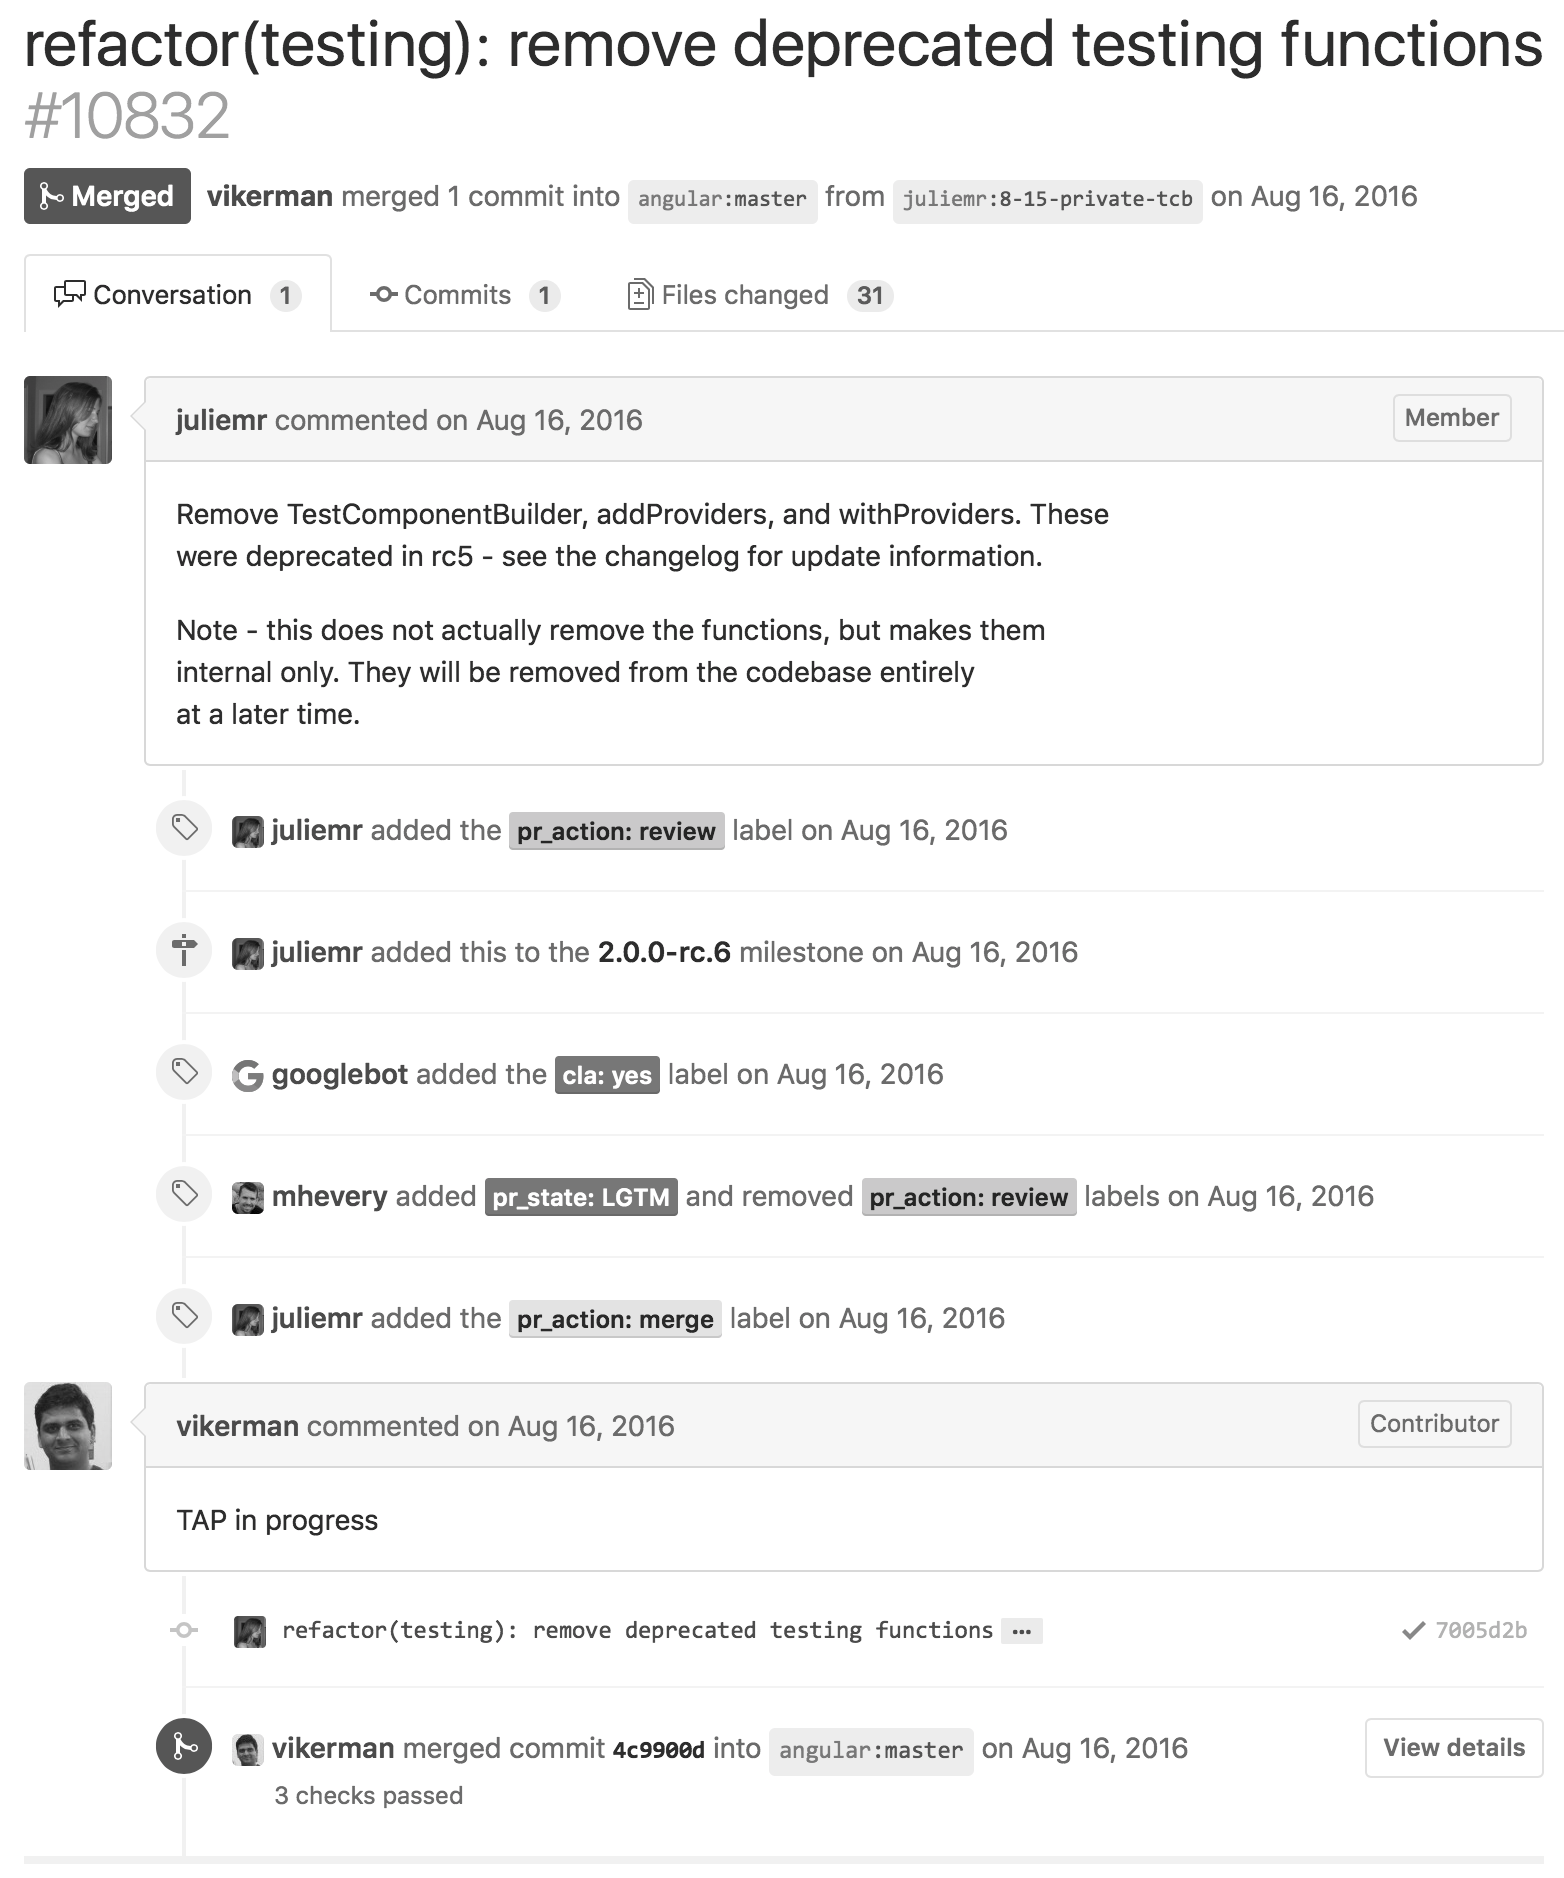
\includegraphics[width=1\columnwidth]{graphics/PRexample.png}
\caption{Screenshot of \ac{PR}}
\label{figure:prexample}
\end{figure}

The entire processing chain is summarized in Figure~\ref{figure:flowchart_processing}. In the actual implementation, a parallel architecture was used as well as a database backed prioritized queue to better handle the large amount of \ac{PR}s and repositories while allowing for pausing and restarting of the processing engine.\footnote{The entire code of the processing chain can be found at https://github.com/pascalwhoop/github-gender-processing}

\begin{figure*}[!t]
\centering
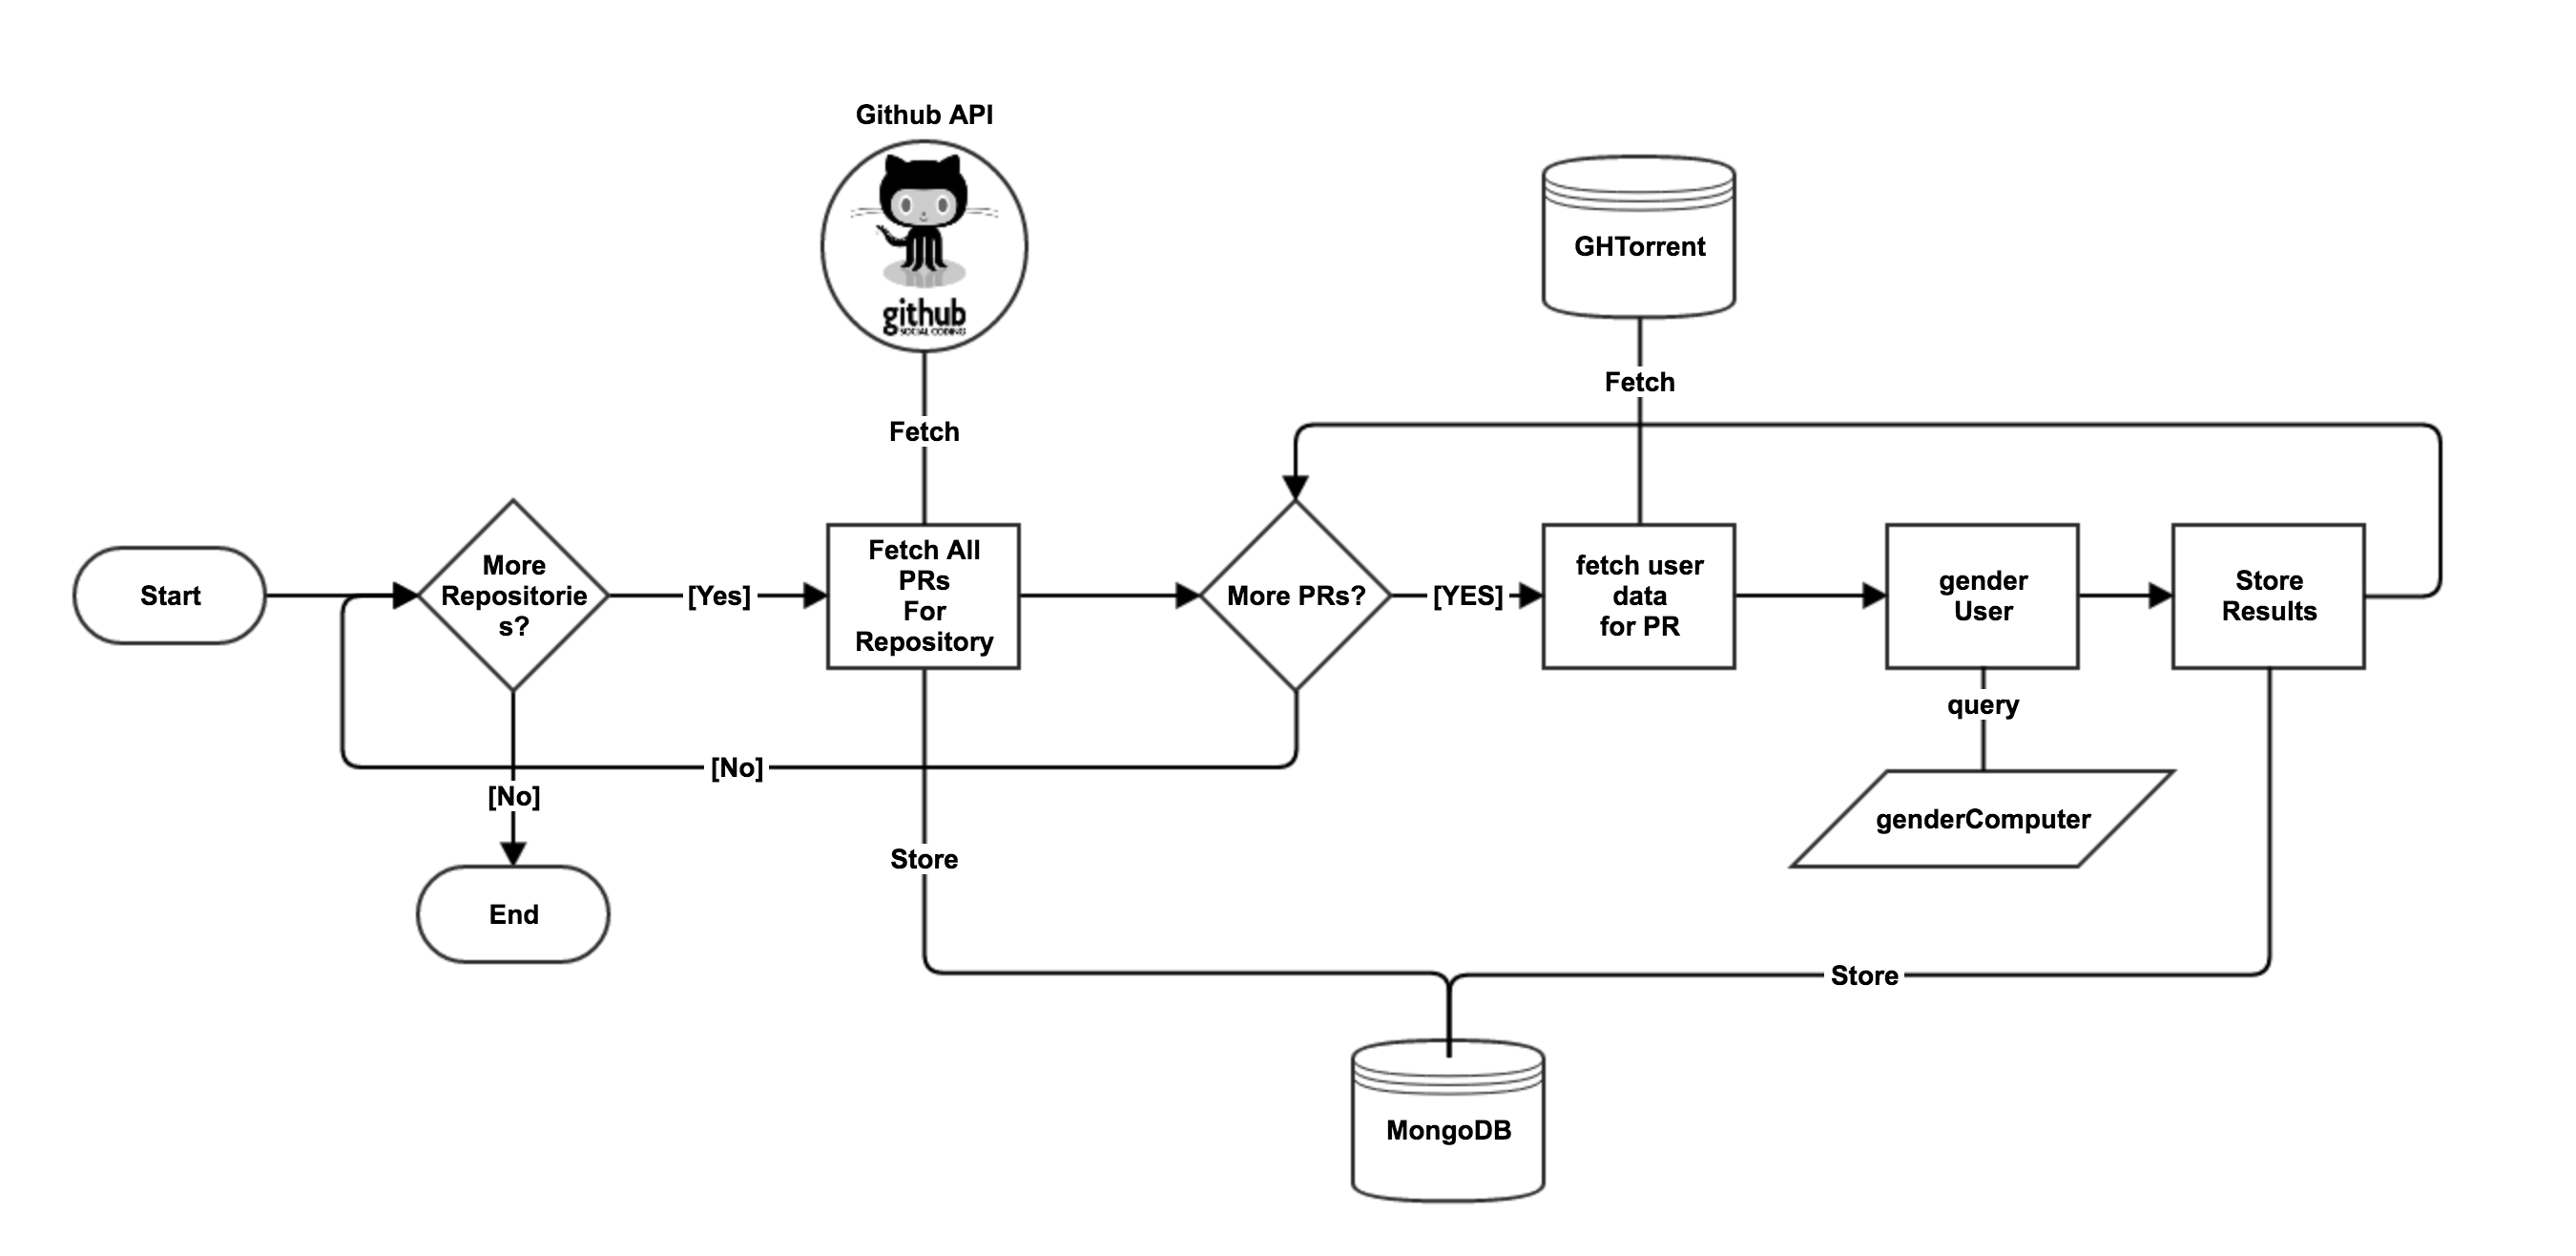
\includegraphics[width=\textwidth]{graphics/flowchart_processing.png}
\caption{Flowchart describing the processing flow}
\label{figure:flowchart_processing}
\end{figure*}



After the data preparation, the analysis of the data can be performed. To analyze the differences between projects, all past \ac{PR}s of each project are analyzed. For each \ac{PR}, a tuple of id, repository, creator's gender and merge result is created.

%\subsection{Determining project culture}

%========

%PROJECT CULTURE

%=========





%\section{Data Processing} % (fold)
%\label{sec:data_processing}

% section data_processing (end)

%\begin{enumerate}
%	\item iterate over \ac{PR}s
%	\item for each: determine if accepted / rejected
%\end{enumerate}


\section{Results}

A total of 43,039 users and 183,249 \ac{PR}s were analyzed.
The \lstinline|genderComputer| determined the gender of 63.23\% of the total number of users, determining the gender from their provided real name, their username and then their email address in descending order of result prioritization.
The success rate was higher than those reported by \citeauthor{vasilescu:2012:6542459}, most likely because we focused on \ac{PR}s that were in the largest projects on GitHub. Users in these repositories have more complete profiles in comparison to the large long tail of small and empty or personal projects, with 66.15\% of all users analyzed having entered their name to their profiles, although its an optional field. Of the gendered users, a total of 1985 or 7.27\% were female which is slightly lower than the 9\% reported by \cite{vasilescu:2012:6542459}. Women have created on average 4.18 and men 4.69 \ac{PR}s.

Using the gender linked \ac{PR}s and user profiles, summary statistics were created for each project. A sample of these results is shown in Table~\ref{table:sampledata}.


\begin{table}[!t]
	\renewcommand{\arraystretch}{1.3}
	\caption{Sample of repo data}
	\label{table:sampledata}
	\centering

	\begin{tabular} { l | l | l | l  }
		\textbf{Attribute} 			& 	\textbf{angular}		&	\textbf{docker}	&	\textbf{ghost}	\\ \hline

		PR Count		&2369	&	15146&1738 \\
		PR merged count 	&720	&	12024&1323 \\
		PR declined count 	&1649	&	3122 &415  \\
		Male PRs		&1586	&	9445 &867  \\
		Female PRs		&161	&	980  &280  \\
		unknown gender PRs	&622	&	4721 &591  \\
		male merged count  	&494	&	7664 &640  \\
		male declined count	&1092	&	1781 &227  \\
		female merged count	&66	&	820  &256  \\
		female declined count	&95	&	160  &24   \\

%	\textbf{$p $} 		& \multicolumn{3}{ |c| }{\textless0.005}	\\ \hline
%	\textbf{$\chi^2$}	&8.98	&28.80	& 38.62			\\ \hline
%	\textbf{$\alpha$}	& \multicolumn{3}{ | c | }{7.879}		\\  \hline

	\end{tabular}
\end{table}

To analyze the results, the chi-squared test for statistical significance was used. This test offers the ability to determine correlation between two variables  \cite[p.102ff.]{chi2016springer}. In the study the correlation between the expected number of declined or merged \ac{PR}s for each gender and the actual number was to be determined.

To evaluate correlation and calculate statistical significance, the chi-squared pearson test requires the calculation of a test statistic $ \chi^2 $ which is then compared to a chi-squared probability of a defined probability barrier (0.005 in this study). The formula for calculating the test statistic is visible in Equation~\ref{equation:statistic}.

\begin{equation}
    \label{equation:statistic}
\chi^2= \sum_{i=1}^{r} \sum_{j=1}^{c} \frac{(O_{i,j} - E_{i,j})^2}{E_{i,j}}
\end{equation}

In this study, both $r$ and $c$ were 2, causing $df = 1$ and $\alpha = 7.879$ with $\chi^2(p<0.005, df=1)$.

Out of the 100 projects analyzed, 53 offered usable results that complied with the rule of having a count of at least 5 in each of the fields used for the $\chi^2$ test \cite[p.104]{chi2016springer}. Of those 53 projects, 18 projects had results that were statistically significant with $\chi^2(p<0.005, df=1)$. The results of those 18 projects are summarized in Table~\ref{table:results}.


\begin{table}[!t]
         \renewcommand{\arraystretch}{1.3}
         \caption{Results of statistically significant projects}
         \label{table:results}
         \centering

         \begin{tabular} {  l | l | l | l | l}
		 \textbf{Project}        &       \textbf{Languages}             &       $\chi^2$        &       $p-value$                       &       $n$             \\ \hline
                 docker                  &       Go                             &       28.803                  &       2.46302E-06             &       15146           \\
                 angular.js              &       \ac{JS}                     	&       21.782                  &       7.23989E-05             &       6570            \\
                 swift                   &       Swift                          &       27.285                  &       5.12939E-06             &       6699            \\
                 node                    &       \ac{JS}			&       105.113                 &       1.23554E-22             &       5721            \\
                 elasticsearch           &       Java                           &       10.378                  &       0.0156108               &       4412            \\
                 react                   &       \ac{JS}                      	&       35.257                  &       1.07507E-07             &       4350            \\
                 react-native            &       \ac{JS},Java,Obj-C     	&       8.021                   &       0.045586391             &       4518            \\
                 django                  &       Python                         &       39.850                  &       1.14627E-08             &       3427            \\
                 atom                    &       CoffeeScript                   &       32.610                  &       3.893E-07               &       2973            \\
                 electron                &       C++                            &       14.238                  &       0.002598504             &       2714            \\
                 angular                 &       TypeScript                     &       8.980                   &       0.029554946             &       2369            \\
                 tensorflow              &       C++,Python                     &       11.875                  &       0.00782457              &       2367            \\
                 Ghost                   &       \ac{JS}                      	&       38.624                  &       2.08483E-08             &       1738            \\
                 discourse               &       Ruby,\ac{JS}	         	&       8.341                   &       0.039460895             &       1843            \\
                 moment                  &       \ac{JS}                      	&       27.567                  &       4.47637E-06             &       1234            \\
                 Modernizr               &       \ac{JS}                      	&       9.299                   &       0.025571851             &       479             \\
		 \parbox[t]{1.7cm}{free-program\\ming-books}  &       None                           &       21.220                  &       9.47533E-05             &       414             \\ \hline

                                 \multicolumn{4}{  c  }{$\alpha = 0.005$}                                                                \\
                                 \multicolumn{4}{  c  }{  $\chi^2_{(0.95;1)} = 7.879 $  }                                                \\ \hline
	\end{tabular}
\end{table}

As \citeauthor{genderdiff:2016} noted, simple statistical significance is not a good indicator for such results alone and therefore, those projects with a strong statistical significance have been controlled for the Pearson correlation. The results are summarized in Table~\ref{table:pearsonoutliers}. Negative values describe projects in which women are less likely to have their PR accepted and positive values describe projects in which women are more likely to have their PR accepted.

Referring back to the perils of mining GitHub defined by \citeauthor{perils-github:2015}, the results need to be controlled for peril 4, 6 and 8. Peril 4 (usage of GitHub for non-software projects) is applicable to 'free-programming-books', the last project in Table~\ref{table:results} which is a information collection project using GitHub as a host.

Peril 6 (not all projects use \ac{PR}s) is applicable to a few of the projects investigated, however non of the statistically significant results is affected. This is intuitive, since a large amount of \ac{PR}s is required to ensure statistical significance which in itself is what needs to be controlled for.

Peril 8 (most \ac{PR}s appear as non-merged but were using non GitHub methods) can be observed in several projects. For this the average merge rate per project was a good indicator to find those projects that tend to not use GitHubs \ac{PR} system systematically. "angular.js", "node", and "jquery" all had a merging average of 15\% or less with an average of 50.24\% across all \ac{PR}s. While jquery is a more mature project, predating GitHub, angular.js has been developed mainly on GitHub infrastructure which therefore suggests that this project has not used the \ac{PR} concepts or has used other forms of including contributions (such as commit squashing or Git based git-request-pull commands). This has changed with "angular", which is the second major version of angular.js, which has a 30\% \ac{PR} merge average, a 23\% increase. At this point, a correlation analysis between gender and type of \ac{PR} acceptance technique was not performed, referring to the work of \citeauthor{genderdiff:2016} who have not identified this as a possible reason.

\begin{table}[!t]
\renewcommand{\arraystretch}{1.3}
          \caption{Pearson correlation for selected outliers}
          \label{table:pearsonoutliers}
          \centering

          \begin{tabular} {  l | l | l}
		  \textbf{Project}        &       $\rho_{merged,gender}$		&	$n$		\\ \hline
		moment			&	-0.217					&	1,234		\\
		node			&	-0.184					&	5,721		\\
		django			&   -0.173					&   3,427		\\
		atom			&	-0.169					&	2,973		\\
		react			&	-0.146					&	4,350		\\
		jquery			&	-0.138					&	2,169		\\
		electron		&	-0.121		  			&	2,714		\\
		angular.js		&	-0.074					&	6,570		\\
		angular			&	 0.008					&	2,369		\\
		Ghost			&	 0.112 					&	1,738		\\

         \end{tabular}

\end{table}

\subsection{Discussion}

The quantitative results of the gender bias on GitHub have shown an interesting picture. While previous research has found a gender bias analyzing the overall \ac{PR} acceptance rate of most repositories on GitHub, the results that focus on a project level difference have offered a more detailed picture. While most repositories only offered statistically insignificant results, 18 showed a significant bias and 7 projects have shown a Pearson correlation between merge result and gender of $\rho > 0.10$, exceeding those results observed by \citeauthor{Davison2000225} with an average Pearson correlation of $\rho = 0.07$ between gender and job selection. The reasons for these biases can be various but ultimately require a qualitative inspection of the projects noted to investigate social differences between them. At first, the project "Ghost", which is the only project having a significant and strong bias towards female acceptance probability, stands out. It is also the project with the highest female participation rate (24\% of all \ac{PR}s were created by female users). This however is due to one active woman, accounting for 86.79\% of all female \ac{PR}s. All other projects either showed insignificant results or were biased towards male contributions.

This leads to the conclusion that the overall bias observed in previous research includes some examples of projects which tend to have a rather strong bias towards male contribution acceptance. Although the work of \citeauthor{Vasilescu:2015:GTD:2702123.2702549} regarding gender and tenure diversity and project success is hardly applicable to the 100 most successful projects on GitHub, the results still leave room for interpretation. The projects listed in Table~\ref{table:pearsonoutliers} all, with the previously described exception of Ghost, show strong biases towards male contributions.

An interesting development can be observed between the two projects angular.js and angular, the latter being the second version of the first one. This allows for a coincidental observation of a temporal change of bias in a community. $ \rho $ has changed from $ -0.074 $ to $0.008$, effectively eliminating the correlation between gender and merge decision.

\section{Limitations and further research}
The research method introduces a few limitations. Those threats to validity originating from performing empirical research on Git repositories \cite{perils-ms-research:2009} or specifically GitHub data \cite{perils-github:2015} has been considered in the research method and its implications were discussed.

However, this paper has not specifically reprocessed all \ac{PR}s to identify all merges as such but rather relied on the GitHub \ac{API}s data. This might lead to a lower number of merged \ac{PR}s as are actually correct. The results also rely on the results of the \lstinline|genderComputer| regarding the members gender. Some projects could exhibit a strong bias due to very active members creating large amounts of \ac{PR}s whos gender has been wrongly classified. A manual control of the three most active contributors of each of the 18 projects exhibiting significant bias however has not revealed such a case.

Lastly, the study has investigated simply the correlation between gender and merge rate, it does not infer the cause of the \ac{PR} merge decision outcome to be the gender. The literature does however suggest the average female contribution to be of better quality than that of a male possibly due to the survivorship bias observed with female software developers \cite{genderdiff:2016}.


\section{Conclusion}\label{Conclusion}

The observed results of overall bias with some outliers towards more significant bias against women are logical, as they describe a similar picture as \cite{genderdiff:2016}, enriching these results with a higher precision on a project level and showing outliers on this level of detail. Further qualitative research should now be able to investigate a small number of specific projects and determine why they are more biased than others and compare the results with those that do not exhibit bias, such as the "rails" and "kubernetes" projects. This work therefore pinpoints a small number of projects that seem to most probably hold revelations about what influences gender bias in \ac{OSS}. Best practices from these projects could help to slowly transform many other sociometric superstar projects into purely meritocratic communities, which by the laws of network theory would then have strong effects on many smaller projects. The goal of a purely bias free community has both ethical and economical motivations and as such should be pursued further by the community as a whole.



\acrodef{F/LOSS}{free/libre/open source software}
\acrodef{FLOSSPOLS}{Free/Libre and Open Source Policy Support}
\acrodef{OSS}{Open Source Software}
\acrodef{RDBMS}{Relational Database Management System}
\acrodef{JSON}{JavaScript Object Notation}
\acrodef{JS}{JavaScript}
\acrodef{API}{Application Programming Interface}
\acrodef{csv}{comma separated values}
\acrodef{RCA}{Relational Covariate Adjustment}
\acrodef{PR}{pull request}




%Bibliography
\bibliographystyle{IEEEtranN}
\bibliography{dt_references}

\end{document}
